\documentclass{beamer}
%
% Choose how your presentation looks.
%
% For more themes, color themes and font themes, see:
% http://deic.uab.es/~iblanes/beamer_gallery/index_by_theme.html
%
\mode<presentation>
{
  \usetheme{Madrid}      % or try Darmstadt, Madrid, Warsaw, ...
  \usecolortheme{beaver} % or try albatross, beaver, crane, ...
  \usefonttheme{serif}  % or try serif, structurebold, ...
  \setbeamertemplate{navigation symbols}{}
  \setbeamertemplate{caption}[numbered]
} 

\usepackage[english]{babel}
\usepackage[utf8]{inputenc}
\usepackage[T1]{fontenc}
\usepackage{graphicx}
\usepackage{caption}
\usepackage{wrapfig}
\usepackage{tikz}
\usetikzlibrary{shapes,snakes,arrows, chains, positioning, shapes.geometric, shapes.symbols,calc,shadows}
\usepackage{pgfplots}

%tikzxommand
\def\centerarc[#1](#2)(#3:#4:#5)% Syntax: [draw options] (center) (initial angle:final angle:radius)
{ \draw[#1] ($(#2)+({#5*cos(#3)},{#5*sin(#3)})$) arc (#3:#4:#5); }


%commands
\newcommand{\C}{\mathbb{C}}
\newcommand{\CP}{\mathbb{CP}}
\newcommand{\CH}{\mathbb{CH}}
\newcommand{\R}{\mathbb{R}}
\newcommand{\Sp}{\mathbb{S}}
\newcommand{\Hy}{\mathbb{H}}
\newcommand{\p}{\partial}
\newcommand{\ddb}{\partial\bar{\partial}}
\newcommand{\mathcolorbox}[2]{\colorbox{#1}{$\displaystyle #2$}}

\DeclareMathOperator{\Ric}{Ric}
\DeclareMathOperator{\Hess}{Hess}

\newcommand*\circled[1]{\tikz[baseline=(char.base)]{
		\node[shape=circle,draw,inner sep=1pt, fill=orange!40] (char) {#1};}}


\title[]{Interview at University of Loughborough}
\author{Martin de Borbon}
\institute[KCL]{King's College London}
\date[17 January]{17 January, 2023}

\begin{document}
\tikzset{pics/segment/.style args=
	{angle #1 left #2 right #3}{
		code={\draw[rotate=#1] (180:#2)--(0:#3);}}} 
	
\begin{frame}
  \titlepage
\end{frame}

%Uncomment these lines for an automatically generated outline.
%\begin{frame}{Outline}
%  \tableofcontents
%\end{frame}

\section{introduction}

\begin{frame}{Plan}
	\begin{center}
	\begin{itemize}
		\item \textbf{Part I:} Field of research: Geometry
		\vspace{5mm}
		\item \textbf{Part II:} Teaching experience and vision for work at Loughborough
	\end{itemize}	
	\end{center}	
\end{frame}

\section{PART I}

\begin{frame}{Part I: Overview}
\begin{center}
\textbf{MOTIVATION:}
\vspace{4mm}
\begin{itemize}
	\item What is curvature? Constant curvature surfaces
	\item Riemann Surfaces and the Uniformization Theorem
\end{itemize}
\vspace{4mm}
\textbf{MAIN OBJECTS:}
\vspace{4mm}
\begin{itemize}
	\item \emph{K\"ahler-Einstein manifolds}
	\item Metrics with cone singularities
\end{itemize}
\vspace{4mm}
\textbf{MY OWN RESULTS}	
\end{center}
\end{frame}



\subsection{curvature}
\begin{frame}{Curvature of a curve in the plane}
	%\pause
	Let \(c\) be a smooth curve in the plane parametrized by unit speed%\pause
	\[
	c: [a, b] \to \R^2, \hspace{2mm} \|c'(t)\|=1
	\]
%\pause
\begin{figure}
	\begin{center}
		\includegraphics[width=.78\textwidth, scale=0.6]{tcurve.png}
	\end{center}
\end{figure}

\begin{itemize}
	%\pause
	\item \(\mathcolorbox{orange!40}{c''(t) \perp c'(t)}\) %\pause \\
	Proof: differentiate \(1= \langle c'(t), c'(t) \rangle \) to obtain \(\langle c''(t), c'(t) \rangle = 0\)
	%\pause
	\item The curvature \(\kappa\) of the curve at \(c(t)\) is
	\(\mathcolorbox{green!40}{\kappa= \| c''(t)\|}\)
\end{itemize}
\end{frame}

\begin{frame}{Example: the circle}
	%\pause
	\begin{tikzpicture}
		\filldraw (0,0) circle (1pt);
		\draw[] (0,0) circle [radius=3];
		\draw (0,0) -- (2.6,1.5);
		\node at (1.5, 1.2) {\(R\)};
		\node at (6, 2) {\(c(t)= \left( R \cos \left(\frac{t}{R} \right) , R \sin \left(\frac{t}{R} \right) \right)\)};
		\node at (6, .5) {\(0 \leq t \leq 2\pi R\)};
		\node at (6,-1) {\(\mathcolorbox{green!40}{\kappa = \frac{1}{R}}\)};
		
		\filldraw (0,3) circle (2pt);
		\filldraw (-3,0) circle (2pt);
		\filldraw (0,-3) circle (2pt);
		\filldraw (3,0) circle (2pt);
		
		\draw[blue, thick,->] (0,3) -- (-1.5,3);
		\draw[blue, thick,->] (-3,0) -- (-3,-1.5);
		\draw[blue, thick,->] (0,-3) -- (1.5,-3);
		\draw[blue, thick,->] (3,0) -- (3, 1.5);
		
		\draw[red, thick,->] (0,3) -- (0,2);
		\draw[red, thick,->] (-3,0) -- (-2,0);
		\draw[red, thick,->] (0,-3) -- (0,-2);	
		\draw[red, thick,->] (3,0) -- (2,0);		
	\end{tikzpicture}
\end{frame}


\begin{frame}{Gaussian curvature}	
%\pause
\begin{columns}
\begin{column}{.48\textwidth}
	\begin{itemize}
		\item \(S \subset \R^3\) smooth surface
		%\pause
		\item \(p\) point in \(S\)
		%\pause
		\item \(\vec{n}\) unit normal vector at \(p\)
	\end{itemize}
\end{column}	
\begin{column}{.48\textwidth}
\scalebox{.45}{
\begin{tikzpicture}
\filldraw[draw=red, fill=yellow!50, fill opacity=.4] plot [smooth cycle] coordinates {(0,0) (2,2) (7,3) (6,-3) (-1,-1)};
\draw[thick, red, ->] (2.1,.7) -- (1.6,1.2);
\node at (2.1,.7) {\(\bullet\)};
\filldraw[fill=orange!70, fill opacity=.3] (3.2,-.5) -- (5,1.5) -- (.5,2) -- (-1.4,0) -- (3.2,-.5);
\node[scale=1.35] at (2.1, .35) {\(p\)};
\node[red, scale=1.5] at (1.5, 1.35) {\(\vec{n}\)};
\node[scale=1.5] at (-1,1.1) {\(T_pS\)};
\node[scale=1.5] at (5,-1.5) {\(S\)};
\node[scale=1.5] at (0,2.31) {\({\color{red}{\vec{n}}} \perp T_pS\)};
\end{tikzpicture}			
}
\end{column}
\end{columns}
	
\begin{columns}
	%\pause
	\begin{column}{.4\textwidth}
		\scalebox{.45}{
		\begin{tikzpicture}
		\filldraw[draw=red, fill=yellow!50, fill opacity=.4] plot [smooth cycle] coordinates {(0,0) (2,2) (7,3) (6,-3) (-1,-1)};
		\filldraw[fill=blue!40, fill opacity=.4, draw=blue] (1,-1) .. controls (2,1) .. (6,2) -- (6,4) -- (1,3) -- (1,-1);
		\draw[green!50!black, thick] (1,-1) .. controls (2,1) .. (6,2);
		\draw[dashed] (1,-1) -- (1,-3) -- (6,-2) -- (6,2);
		\draw[thick, blue, ->] (2.1,.7) -- (2.7,1.3);
		\draw[thick, red, ->] (2.1,.7) -- (1.6,1.2);
		\node at (2.1,.7) {\(\bullet\)};
		\node[scale=1.5] at (5,-1.5) {\(S\)};
		\node[red, scale=1.5] at (1.5, 1.45) {\(\vec{n}\)};
		\node[scale=1.5] at (2.1, .35) {\(p\)};
		\node[blue, scale=1.5] at (3, 1.6) {$\vec{v}$};
		\node[blue, scale=1.5] at (.7,3.3) {\(P\)};
		\node[green!50!black, scale=1.5] at (5, 1.2) {\(c\)};
		\end{tikzpicture}	
	}	
	\end{column}
\begin{column}{.6\textwidth}
	\begin{itemize}
		%\item \(\vec{v}\) unit tangent vector at \(p\)
		\item \(P\) plane that contains \(\vec{n}\)
		\item \(c\) unit speed curve \(P \cap S\)
		\item \emph{Signed} curvature \(\kappa = \langle c''(0), \vec{n} \rangle\)
	\end{itemize}
\end{column}
\end{columns}	
%\pause
\begin{center}
	The Gaussian curvature \(K\) of \(S\) at \(p\) is \(\mathcolorbox{green!40}{K = \kappa_{\min} \cdot \kappa_{\max}}\)
\end{center}
\end{frame}


\begin{frame}{Examples}
	%\pause
	\begin{columns}
		\begin{column}{.48\textwidth}
			\centering Sphere
			\begin{center}
			\scalebox{.6}{
				\begin{tikzpicture}
				\filldraw[draw=green!50!black, thick, fill=yellow!30] (0,0) circle [radius=3];
				\filldraw (0,0) circle (2pt);
				\draw[dashed] (0,-3) to[bend right, out=-90, in=-90] (0,3);
				\draw[green!50!black, thick] (0,-3) to[bend left, out=90, in=90] (0,3);
				\draw[red, thick, ->] (0,3) -- (0,2);
				\draw (0,0) to (3,0);
				\node[red] at (0,1.7) {\(\vec{n}\)};
				\node[scale=1.5] at (1.4,.3) {\(R\)};
				%\draw (0,0) circle [x radius=1, y radius=3];
				\end{tikzpicture}
			}	
			\end{center}
			
		\[\mathcolorbox{green!40}
		{K = \frac{1}{R} \cdot \frac{1}{R} = \frac{1}{R^2}}
		\]
		\end{column}
		
		\begin{column}{.48\textwidth}
			\centering Negative curvature
			\begin{figure}
			\scalebox{.5}{
				\begin{tikzpicture}
				\begin{axis}[hide axis]
				\addplot3[surf, fill=blue!20, domain=-1:1] {y^2 - x^2};
				\end{axis}
				\end{tikzpicture}
			}	
			\caption*{\(K<0\)}
			\end{figure}
			
		\end{column}
	\end{columns}
\end{frame}


\begin{frame}{Foundations: Egregium and Gauss-Bonnet}
	%\pause
	\textbf{Gauss's Egregium Theorem:} \(K\) is invariant under isometries  %\pause \\	
	Intrinsic distance determines \(K\), %\pause e.g. 
	\[
	\frac{A(r)}{\pi r^2} = 1 - \frac{K}{12}r^2 + O(r^3) \hspace{4mm} \text{ as } r \to 0
	\]
	where \(A(r)\) is the area of a disc of radius \(r\) centred at \(p\)
	%\pause
	
	\textbf{Gauss-Bonnet Theorem:} \(S\) compact, no boundary
	\begin{columns}
		\begin{column}{.48\textwidth}
	\[
	\mathcolorbox{green!40}{
	\frac{1}{2\pi} \int_S K dA = \chi(S)
	}
	\]			
	\end{column}
\begin{column}{.48\textwidth}
	\begin{center}
	\scalebox{.5}{
	\begin{tikzpicture}
	\draw (0,0) -- (2,0) -- (1,2) -- (0,0);
	\draw (1,2) to (2,1);
	\draw[dashed] (0,0) -- (2,1);
	\draw (2,1) to (2,0);
	\node[scale=2] at (1,-1) {\(\chi = F - E + V =2\)};
	\end{tikzpicture}
}		
	\end{center}
\end{column}
	\end{columns}
	%\pause
		\begin{center}
		\scalebox{.7}{
			\begin{tikzpicture}
			\draw (-5,0) circle [radius=1];
			\draw (-6,0) to[bend right] (-4,0);
			\draw[dashed] (-6,0) to[bend left] (-4,0);
			\node[scale=1.3, blue](b) at (-5,-1.5){\(\chi=2\)};
			
			
			\draw (-1,0) ellipse (2 and 1);
			\draw (-1.5,0) to[bend left] (-.5,0);
			\draw (-1.7,.1) to[bend right] (-.3,.1);
			\node[scale=1.3, blue](b) at (-1,-1.5){\(\chi=0\)};
			
			\draw (5,0) ellipse (3 and 1);
			\draw (3.5,0) to[bend left] (4.5,0);
			\draw (3.3,.1) to[bend right] (4.7,.1);
			\draw (5.5,0) to[bend left] (6.5,0);
			\draw (5.3,.1) to[bend right] (6.7,.1);
			\node[scale=1.3, blue](b) at (5,-1.5){\(\chi=2-2\mathrm{g}<0\)};
			\end{tikzpicture}
		}		
	\end{center}
\end{frame}


\subsection{constant curvature}
\begin{frame}{Constant curvature}
\(3\) model spaces: 
\begin{itemize}
	\item \(\Sp^2\) is the unit sphere, \(K = 1\)
	\item \(\R^2\) is the Euclidean plane, \(K=0\)
	\item \(\Hy^2\) is the \textbf{hyperbolic plane}, \(\mathcolorbox{green!40}{K=-1}\)	
\end{itemize}

			\begin{center}	
	\begin{figure}
		\scalebox{.9}{
			
			\begin{tikzpicture}
			\filldraw[fill=yellow!40, draw=black] (8,1) circle [radius=1.5]; 
			\filldraw (8,1) circle [radius=.05];
			\draw[blue, thick] (8,2.5) arc (180:270:1.5);
			\draw[blue, thick] (8,-.5) arc (0:90:1.5);
			\draw[red, very thick] (6.5,1) -- (9.5,1);
			\node at (8, .7) {\(0\)};	
			\node at (13, 1.5) {\(\{|z|<1\} \subset \C\)};
			\node at (13,.5) {hyperbolic metric $=\frac{4}{(1-|z|^2)^2}|dz|^2$};	
			\end{tikzpicture}	
		}
		\caption*{\textbf{Poincar\'e disc model.} Distances go to infinity as we approach the boundary unit circle \(\{|z|=1\}\). \emph{Geodesics} are circles orthogonal to the unit circle and also diameters through the origin.}
	\end{figure}	
\end{center}
\end{frame}



\begin{frame}{Visualization of the hyperbolic plane}
	\begin{columns}
		%\pause
		\begin{column}{.48\textwidth}
			\begin{center}
				\includegraphics[scale=.3]{hypmen.png}
			\end{center}
		\end{column}
	%\pause
		\begin{column}{.48\textwidth}
		\begin{center}
			\includegraphics[scale=.25]{escher.png}
		\end{center}
	\end{column}
	\end{columns}
	%\pause
	\begin{center}
		\includegraphics[scale=.3]{tractrix.png}
	\end{center}
\end{frame}


\begin{frame}{Constant curvature surfaces}	
\begin{columns}
%\pause	
\begin{column}{.48\textwidth}

\begin{figure}
\scalebox{.7}{				
	\begin{tikzpicture}
	\filldraw[yellow!40] (0,0) -- (1,2) -- (4,2) -- (3,0);
	\draw[very thick, blue, ->] (0,0) -- (1.5,0);
	\draw[very thick, blue] (1.5,0) -- (3,0);		
	\draw[very thick, blue, ->] (1,2) -- (2.5,2);
	\draw[very thick, blue] (2.5,2) -- (4,2);
	\draw[very thick, red, ->] (0,0) to (.5,1);
	\draw[very thick, red] (.5,1) -- (1,2);
	\draw[very thick, red, ->] (3,0) to (3.5,1);
	\draw[very thick, red] (3.5,1) -- (4,2);	
	\end{tikzpicture}				
	}
\caption*{Identify opposite sides of a parallelogram to obtain a flat torus}
	\end{figure}
\end{column}
	%\pause
	\begin{column}{.48\textwidth}
		
		\begin{figure}
				\includegraphics[scale=.4]{octagon.png}
				\caption*{Regular hyperbolic octagon with \(45^{\circ}\) interior angles. Identification yields a hyperbolic surface of genus \(2\).}
		\end{figure}		
\end{column}
\end{columns}	
\end{frame}


\subsection{Riemann surfaces and Uniformization}
\begin{frame}{Conformal maps}
%\pause	
\(F\) is conformal (or \emph{isothermal}) if it preserves angles and orientation

	\scalebox{.7}{
		\begin{tikzpicture}
		\filldraw[draw=black, fill=green!40] (-4,0) circle [radius=1];
		\draw[->] (-4,-.5) to (-4, 1.5);
		\draw[->] (-4.5, 0) to (-2.5, 0);
		\filldraw[draw=black, fill=green!40] (2,0) circle [x radius=1.5, y radius=.8];
		
		\draw[->] (-2.5, 1) to[bend left] (2, 1);
		\node at (0, 2) {\(F\)};
		\draw[draw=red] plot [smooth cycle] coordinates {(0,0) (2,2) (5,2) (4,-1) (-1,-1)};
		\draw[blue, ultra thick, ->] (-3.8,.5) -- (-3.1, .5);
		\draw[blue, ultra thick, ->] (-3.8,.5) -- (-3.8, 1.2);
		\draw[blue, ultra thick, ->, rotate around={45:(2,0)}] (2,0) -- (2.7, 0);
		\draw[blue, ultra thick, ->, rotate around={45:(2,0)}] (2,0) -- (2, .7);
		\node[scale=1] at (4,1.5) {\(S \subset \R^3\)};
		\end{tikzpicture}	
	}	

%\pause
\textbf{Theorem} (Gauss) Every surface has isothermal coordinates
%\pause
\begin{figure}
	\includegraphics[scale=.4]{conformal.png}
	\caption*{\(f\) is conformal \(\iff\) \(f\) is (locally invertible and) \textbf{holomorphic}}
\end{figure}	
\end{frame}


\begin{frame}{Riemann surfaces}
	%\pause
	A Riemann surface is built from pieces of \(\C\) using holomorphic patches
	%\pause
	\begin{figure}
		\includegraphics[scale=.4]{riemsurf.png}
		\caption*{Riemann surface of the function \((1-z^3)^{1/2}\)}
	\end{figure}
\end{frame}


\begin{frame}{Uniformization Theorem}
	%\pause
	\begin{block}{Poincar\'e, Klein \(\sim 1883\)}
		Every compact Riemann surface admits an essentially unique \textbf{conformal} metric of constant curvature \(K\).
	\end{block}
%\pause	
\begin{columns}
	\begin{column}{.48\textwidth}
		Riemann mapping theorem
	\end{column}
	\begin{column}{.48\textwidth}
		\includegraphics[scale=.25]{rmap.png}
	\end{column}
\end{columns}
%\pause
\begin{align*}
	\{\text{Constant curvature metrics}\} &\iff \{\text{Riemann surfaces}\} \\
	\Sp^2, \R^2, \Hy^2 &\iff \CP^1, \C, \mathbb{D}
\end{align*}
\end{frame}


\subsection{KE and cs}
\begin{frame}{K\"ahler-Einstein metrics}
%\pause	
Complex manifolds are glued from open sets in \(\C^n\)	
%\pause
		\begin{columns}
			\begin{column}{.48\textwidth}
			\begin{equation*}
			\lambda \in \R, \hspace{2mm}
			\mathcolorbox{orange!40}{
				\Ric(g) = \lambda \cdot g
			} 
			\end{equation*}		
			\end{column}
			\begin{column}{.48\textwidth}
				\begin{figure}
					\begin{center}
						\includegraphics[width=.48\textwidth]{einstein.jpg}
					\end{center}
				\end{figure}
			\end{column}
		\end{columns}
	
		\begin{itemize}
		%\pause	
		\item Ricci curvature is an average of sectional (Gaussian) curvatures
		%\pause
		\item K\"ahler is a compatibility condition between metric and complex structure 
		(when \(\dim_{\C}=1\) it means conformal)
	\end{itemize}
%\pause
\begin{columns}
	\begin{column}{.3\textwidth}
		\begin{figure}
			\begin{center}
				\includegraphics[width=.7\textwidth]{CalabiYau5.jpg}
			\end{center}
			%\caption*{2D-slice of a quintic CY 3-fold}
		\end{figure}
	\end{column}
	\begin{column}{.6\textwidth}
		\begin{itemize}
			\item Calabi-Yau  manifolds solve \(\Ric=0\)
			\item Example: the  quintic 3-fold 
			\[\{z_0^5+\ldots+z_4^5=0\} \subset \CP^4\]
		\end{itemize}
	\end{column}
\end{columns}
\end{frame}


\begin{frame}{Cone singularities}
%\pause	
\begin{columns}
	\begin{column}{.48\textwidth}
	Fix \(\beta>0\).
	\textbf{The \(2\)-cone of total angle \(2\pi\beta\)}.	
	In polar coordinates
	\[dr^2+ \beta^2 r^2 d\theta^2\]
\end{column}
	\begin{column}{.48\textwidth}
			\begin{center}
			\scalebox{0.5}{	
				\begin{tikzpicture}
				%leftpart
				\filldraw[fill=green!20, draw=blue] (-2,0) -- (0,0) arc (0:220:2) -- (-2,0);
				\centerarc[thick](-2,0)(5:215:.7);
				\centerarc[<->,dashed,thick](-2,0)(225:355:1);
				%middle arrow
				\draw[->,dashed,thick] (1,1) to (3,1);
				%rightpart
				\filldraw[fill=green!20] (4,2) to[bend right] (7,2) -- (5.5,-1) -- cycle;
				\draw[dotted,thick] (4,2) to[bend left] (7,2);
				%nodes
				\node[scale=1.3](a) at (-2,1.1){\(2\pi\beta\)};
				\node[scale=1.3](b) at (0,-.5){identify};
				%\node[fill=red!20,draw,rounded corners, scale=1.5](c) at (-4.5,2.5){\(0<\beta<1\)};
				\end{tikzpicture}
			}
		\end{center}
		
	\end{column}
\end{columns}	
%\pause	
	
	\begin{columns}
		\begin{column}{.38\textwidth}
			\[
			\begin{cases}
			dr^2 + \beta^2\sin^2 r d\theta^2  \\
			dr^2 + \beta^2 r^2 d\theta^2 \\
			dr^2 + \beta^2 \sinh^2r d\theta^2 
			\end{cases}
			\]
		\end{column}
		
		\begin{column}{.58\textwidth}
			\begin{figure}[t]
				\centering
				\scalebox{.7}{
					\begin{tikzpicture}
					\filldraw[fill=green!50, draw=black] (-1,2) -- (0,0) -- (1,2) to[bend left] (-1,2);
					\draw[dashed] (-1,2) to[bend left] (1,2);
					
					\filldraw[fill=green!50, draw=black] (-4,2) to[bend right] (-3,0) to[bend right] (-2,2) to[bend left] (-4,2);
					\draw[dashed] (-4,2) to[bend left] (-2,2);
					
					\filldraw[fill=green!50, draw=black] (2,2) to[bend left] (3,0) to[bend left] (4,2) to[bend left] (2,2);
					\draw[dashed] (2,2) to[bend left] (4,2);
					
					%\node[scale=1.4] at (-3,-.4) {\(K=1\)};
					%\node[scale=1.4] at (0,-.4) {\(K=0\)};
					%\node[scale=1.4] at (3,-.4) {\(K=-1\)};
					
					\node[] at (-3,2.6) {\((2\pi\beta)\sin r\)};
					\node[] at (0,2.6) {\((2\pi\beta)r\)};
					\node[] at (3,2.6) {\((2\pi\beta)\sinh r\)};
					
					\node[] at (-4.1,1) {\(r\)};
					\node[] at (-.8,1) {\(r\)};
					\node[] at (2.6,1) {\(r\)};
					\end{tikzpicture}	
				}
			\end{figure}
		\end{column}
	\end{columns}

\begin{columns}
	%\pause
	\begin{column}{.48\textwidth}
			\begin{figure}
			\scalebox{.7}{
				\begin{tikzpicture}
				\filldraw[fill=yellow!70, draw=black] (-1,-2) to[bend right] (1,-2) to[bend right] (0,0) to[bend right] (-1,-2);
				
				\draw (-.4, -.35) to[bend right] (.4,-.35);
				\draw[dashed] (.4,-.35) to[bend right] (-.4,-.35);
				
				\draw (-1, -1.5) to[bend right] (-.6, -2.2);
				\draw[dashed] (-1, -1.5) to[bend left] (-.6, -2.2);
				
				\draw[dashed] (1, -1.5) to[bend right] (.6, -2.2);
				\draw (1, -1.5) to[bend left] (.6, -2.2);
				
				\node[] at (0,-.7) {\(2\pi \beta\)};
				\end{tikzpicture}		
			}
		\caption*{Double of spherical triangle. Metric on \(\CP^1\) with \(3\) cone points.}
		\end{figure}
	\end{column}
%\pause
	\begin{column}{.48\textwidth}
			\begin{figure}
			\scalebox{.5}{
				\begin{tikzpicture}
				\draw (0,0) -- (2,0) -- (2,2) -- (0,2) -- (0,0);
				\draw (2.7,.7) -- (2.7,2.7) -- (.7,2.7);
				\draw[dashed] (0.7,2.7) -- (0.7,0.7) -- (2.7,0.7);
				\draw[dashed] (0,0) -- (.7,.7);
				\draw (0,2) -- (.7,2.7);
				\draw (2,0) -- (2.7,.7);
				\draw (2,2) -- (2.7, 2.7);
				\end{tikzpicture}
			}
		\caption*{Flat metric on \(\CP^1\) with \(8\) cone points  \(\beta=3/4\).}
		\end{figure}
	\end{column}
\end{columns}
\end{frame}

\subsection{my own work}	
\begin{frame}{My own work}
	%\pause
	\begin{columns}
		\begin{column}{.48\textwidth}
			Calabi-Yau metrics with cone singularities along a smooth complex curve \(C \subset \C^2\) \\
			(PhD at Imperial College London supervised by Simon Donaldson)
		\end{column}
		\begin{column}{.48\textwidth}
				\begin{figure}
				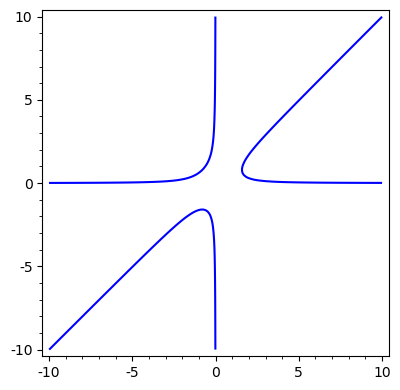
\includegraphics[scale=.3]{cubic.png}
			\end{figure}
		\end{column}
	\end{columns}
%\pause
\begin{columns}
	\begin{column}{.48\textwidth}
			\begin{center}
			\scalebox{0.5}{
				\begin{tikzpicture}
				%lines
				\draw (-4,0) to (4,0);
				\draw (-4,-2) to (2,4);
				\draw (4,-2) to (-2,4);
				\draw (0, -2) to (0,4);
				\draw (-4,-2/3) to (3,5/3);	
				\draw (4,-2/3) to (-3,5/3);
				
				%nodes
				\draw (-2,0) node [shape=circle,draw, fill=red, scale=.5] (asd) {};
				\draw (2,0) node [shape=circle,draw, fill=red, scale=.5] (asd) {};
				\draw (0,2/3) node [shape=circle,draw, fill=red, scale=.5] (asd) {};
				\draw (0,2) node [shape=circle,draw, fill=red, scale=.5] (asd) {};
				\draw (-1,1) node [shape=circle,draw,fill=blue,scale=.5] (asd) {};
				\draw (0,0) node [shape=circle,draw,fill=blue,scale=.5] (asd) {};
				\draw (1,1) node [shape=circle,draw,fill=blue,scale=.5] (asd) {};
				
				%labels
				\draw  (0.4,-1.9) node (asd) [scale=.9] {\(H_{23}\)};
				\draw  (3.4, 1.8) node (asd) [scale=.9] {\(H_{34}\)};
				\draw  (-3.4,1.8) node (asd) [scale=.9] {\(H_{24}\)};
				\draw  (-2,3.5) node (asd) [scale=.9] {\(H_{12}\)};
				\draw  (2,3.5) node (asd) [scale=.9] {\(H_{13}\)};
				\draw  (1,-.3) node (asd) [scale=.9] {\(H_{14}\)};
				%\draw  (-2.7, 2.7) node (asd) [scale=1.1, color=red] {\((\mathbf{CP}^2, \sum_{i<j} \mu_{ij} L_{ij} ) \)};
				\end{tikzpicture}
			}
		\end{center}
	\end{column}
\begin{column}{.48\textwidth}
	Fubini-Study metrics with cone singularities along the braid arrangement \(\{z_i=z_j\} \subset \CP^n\) \\
	(joint with Dmitri Panov)
\end{column}
\end{columns}
\end{frame}

\section{PART II}

\begin{frame}{Part II: Overview}
	\begin{itemize}
		\item Teaching
		\vspace{5mm}
		\item Mentorship
		\vspace{5mm}
		\item Vision for work at Loughborough
	\end{itemize}
\end{frame}


\begin{frame}{Teaching experience}
	\begin{itemize}
		\item (2015--2017) National University of San Luis, Argentina. \\ Lecturer: Sequences and Series, Principles of Mathematical Analysis, PDEs, Representation of Finite Groups, and Computational Algebraic Geometry 
		\vspace{2mm}
		\item (2017-2019) Aarhus University, Denmark. PhD lecture course on K\"ahler Geometry. Parts of the master courses:  Riemannian Geometry and Riemann Surfaces.
		\vspace{2mm}
		\item (2021-2022) King's College London. Tutorials on Geometric Topology. Nominated to Outstanding Teaching Assistant Awards:
		\begin{center}
			\emph{"Very clear explanations, pausing frequently to make sure we have understood and for questions. Breaks down difficult concepts and overall an excellent tutor!"}
		\end{center}
	\end{itemize}
\end{frame}

\begin{frame}{Mentorship}
	\begin{itemize}
		\item (2018-2019) Co-supervisor of Jorge Bravo's master thesis \emph{On Calabi-Yau conifolds} at Aarhus University. He is now a PhD student at Technical University of Denmark.
		\vspace{5mm}
		\item (2021-2022) Supervisor of Dylan Prod'homme-Bennett's master thesis \emph{Hodge theory} at King's College London. His thesis was considered for the J G Semple departmental prize. He is now a Crude Oil Derivatives Trader at Onyx Commodities.
	\end{itemize}
\end{frame}


\begin{frame}{Vision for work at Loughborough}
	\begin{center}
	\textbf{RELATIONS TO RESEARCH IN PLACE}
	\begin{itemize}
		\item Algebraic Geometry: birational geometry, Fano varieties
		\item Differential Geometry: special holonomy, web geometry
		\item Integrable Systems: KZ equations, hyperplane arrangements, Frobenius manifolds
		\item Geometric Analysis, links to the Analysis and PDEs Group \\ (e.g. microlocal analysis)
	\end{itemize}	
	\textbf{ONGOING COLLABORATIONS}
	\begin{itemize}
		\item Ronan Conlon, University of Texas at Dallas
		\item Dmitri Panov, King's College London
		\item Cristiano Spotti, Aarhus University
	\end{itemize}
	\textbf{GRANT APPLICATIONS}
	\begin{itemize}
		\item New Investigator Award, EPSRC
	\end{itemize}	
	\end{center}
\end{frame}

\begin{frame}
	\begin{center}
		\huge
		\textbf{
		{\color{blue!50!black}{THANK YOU!}}
		}
	\end{center}
\end{frame}

\end{document}
